\label{appendix:stimgen}
% Stimulus generator library by Giugliano and Arsiero
\lstset{ 
  backgroundcolor=\color{light_gray},  
  basicstyle = \tiny\ttfamily,       % the size of the fonts that are used for the code
  breakatwhitespace = false,        % sets if automatic breaks should only happen at whitespace
  breaklines=true,
  % sets the caption-position to bottom
  captionpos=b, 
  frame=none,                   % adds a frame around the code
  numbers=none,                   % where to put the line-numbers; possible values are (none, left, right)
  tabsize=4
}

\floatstyle{ruled}
\newfloat{example}{thp}{lop}
\floatname{example}{Example}

\section{Introduction}

\paragraph{}
This reference manual constitutes the documentation of the ANSI-C library and executables of the project
\textbf{\textit{Create Stimulus}}. It is based on the previous \textbf{\textit{Generate Trial}} project, originally
developed in the context of the \textit{MeeDuck} and \textit{MauQuack} software suits during the period 2001-2005 by
Drs. M. Giugliano and M. Arsiero at the University of Bern, Switzerland. Such a library and associated executable(s)
support and implement the decoding of a \textit{meta-language} for the computer-synthesis (of a class of) digital
waveforms through its interpretation and conversion into raw numeric time series data. These \textbf{waveforms} are
composed by the \textbf{juxtaposition} of a set of elementary \textbf{subwaveforms}, ad/or of their algebraic
composition. The meta representation has the obvious advantage of a compact description, independent of the waveform
length, the actual discretization/sampling interval, and the D/A quantization resolution. Other advantages are the
little disk storage required and the relative ease of editing and post-processing by ad-hoc softwares (i.e. waveform
editors).

\section{Waveforms and subwaveforms}
\paragraph{}
The raw data output from the \textbf{\textit{Create Stimulus}} library and executable(s) is a sequence of numeric
samples (i.e. double precision floating point values), available for the subsequent D/A conversion in a
stimulus-response probing system, e.g. to impose a particular evolution to a time-varying physical variable, let's say
the stimulation current to be injected in an electronic circuit at a certain node. Such a sequence of numeric samples
is a \textbf{waveform}. However, its specification / disk storage / actual synthesis / etc. does not involve actual
data samples, one for each sampling interval, but instead it is in the form of a \textbf{high-level abstract
description, made of a string of characters}. These are always in multiple of 12 numerical elements, separated by an
arbitrary number of spaces or tab characters. It thus follows that looking at such a string in terms of blocks of 12,
one is actually referring to a time range in the waveform where some of the properties of the overall waveforms are
stationary by definition. One example, for a single \textbf{elementary subwaveform} is given below, where the name of
each field has been indicated.

\begin{center}
\footnotesize\ttfamily
\begin{tabular}{rrrrrrrrrrrr}
[T & CODE & P1 & P2 & P3 & P & P1 & FIXSEED & MYSEED & SUBCODE & OPERATOR & EXPON]
\end{tabular}
\end{center}
	
\paragraph{}
By this definition, we consider a \textbf{waveform} as always subdivided in a series of temporal intervals $i=1,2,3,...$
each lasting \textbf{$T_1$} and each isomorphic to a specific \textbf{subwaveform templates} 
(i.e. as in a piece-wise parametric decomposition). A subwaveform may be \textbf{\textit{elementary}} (e.g. a
\textbf{DC} value lasting for \textbf{$T=3$} seconds, a \textbf{sinusoidal} oscillation
lasting \textbf{$T=5$} seconds, a \textbf{random} noisy signal lasting
\textbf{$T=3$} seconds, etc.) or resulting from the \textbf{\textit{algebraic composition}} of
elementary subwaveforms (e.g. 5 seconds of a noise whose mean is modulated in time as a sinusoidal oscillation).

\paragraph{}
Let's for simplicity consider first only the existence of elementary subwaveforms. As an example, we consider a waveform
made of 4 subwaveforms. As already mentioned, \textbf{each subwaveform is specified as a string of 12 numbers
[. . . . . . . . . . . .] }(see above). Then, the waveform resulting from \textbf{4} subwaveform is simply the
\textbf{linear juxtaposition of 4 x 12 numbers}: \textbf{[. . . . . . . . . . . .] [. . . . . . . . . . . .] [. . . . .
. . . . . . .] [. . . . . . . . . . . .]}. In this example, the \ brackets have been used here only for clarity, as
they are neither necessary nor required. In addition a carriage return is needed as a special separator character
between each value defining a subwaveform or between subsequent subwaveforms.

\paragraph{}
The very first element out of the 12 numbers characterizing each subwaveform is called \textbf{DURATION} and it encodes
the temporal duration \textbf{T} of the subwaveform. Therefore it is possible to infer the overall duration of any
waveform, composed by many subwaveforms, by simply adding together the first elements of each group of subsequent 12
numbers, e.g.:

\begin{center}
\begin{tabular}{rrrrrrrrrrrr}
$T_{1}$ & - & - & - & - & - & - & - & - & - & - & - \\
$T_{2}$ & - & - & - & - & - & - & - & - & - & - & - \\
$T_{3}$ & - & - & - & - & - & - & - & - & - & - & - \\
$T_{4}$ & - & - & - & - & - & - & - & - & - & - & - \\
\end{tabular}
$$T_{total}=T_1+T_2+T_3+T_4$$
\end{center}

\bigskip
	
\paragraph{}
The list of possible numerical values for the field \textbf{CODE}, thus of elementary subwaveforms, is reported below:

\begin{enumerate}
\item DC, constant value, waveform
\item Ornstein-Uhlenbeck stochastic process realization
\item Sinusoidal waveform
\item Square wave, with zero mean
\item Saw tooth wave, with zero mean
\item Sine waveform with frequency sweep
\item Ramp waveform, increasing or decreasing slope
\item Poisson / regular unipolar square pulses
\item Poisson / regular unipolar exponentially decaying pulses
\item Poisson / regular bipolar square pulses (zero mean)
\item Uniformly distributed stochastic process realisation
\item Double exponential decay (Alpha waveform)
\end{enumerate}

\bigskip

\paragraph{}
Because this identifier is a simple integer, the extension of the library to other elementary subwaveforms is
straightforward. However, it will become clearer how a very large variety of waveforms can be made with just 10
elementary types and their arithmetic combination.

\paragraph{}
The information encoded in each of the remaining 10 elements of each 12-elements (sub)string, which describes as we
already said any subwaveform, has a context-dependent meaning: it depends on the \textbf{CODE} and on other
considerations. In the next section, we first examine each elementary subwaveform, its parameters, and their encoding
into the corresponding 12-elements (sub)string.


\section{Elementary subwaveforms}

\paragraph{}
In this section we examine all the possible elementary subwaveforms, introducing the formalism for their full
specification. As already stressed in the previous section of this document, the purpose of such a compressed
meta-representation is to specify/store only the \textbf{\textit{parameters}} necessary to identify the actual
subwaveform, without the need of specifying/storing explicitly the entire time series, sample by sample. With
decreasing cost of storage capacity this may be of limited interest, but its impact on the (implicit) fast
composition/design of a new waveform is obvious.

\subsection{DC elementary subwaveforms}
\paragraph{}
The family of DC elementary subwaveforms is defined by just \textbf{two} parameters: its \textbf{duration} and its
\textbf{amplitude}, according to the following mathematical expression:
\begin{center}
$ f(t) = P_1$ for all times $t \in [t_0:t_0 + T]$
\end{center}

\paragraph{}
The string that identifies this DC elementary subwaveform consists in 12 distinct numerical values, but only 2 of them
are relevant to parametrize the actual trace. Let's ignore \textbf{\textit{EXPON}} for a moment, and let's indicate
with a short segment \textbf{\textit{{}-}} element of the string that are irrelevant for the identification of the DC
elementary subwaveform:

\begin{center}
\footnotesize\ttfamily
\begin{tabular}{rrrrrrrrrrrr}
[T & 1 & P1 & - & - & - & - & - & - & - & - & EXPON]
\end{tabular}
\end{center}

\paragraph{}
The first field of the 12-values string contains the \textbf{duration (in seconds)} of the subwaveform, while the second
field encodes its identifier (i.e. the code - in this example ``1'' corresponds to the DC type). The third field, named
\textbf{$P_1$} takes here the meaning of the only other parameter that the DC
subwaveform requires, i.e. its \textbf{amplitude value (in arbitrary units)}. The remaining fields needs to be
specified as they cannot be left blank, but their actual numerical value (i.e. set to 0 by convention) is ignored.

\begin{example}
\begin{center}
\footnotesize\ttfamily
\begin{tabular}{rrrrrrrrrrrr}
2.5 & 1 & 0.0 & 0 & 0 & 0 & 0 & 0 & 0 & 0 &0 & 1 \\
5.0 & 1 & 2.0 & 0 & 0 & 0 & 0 & 0 & 0 & 0 & 0 & 1 \\
2.5 & 1 & 0.0 & 0 & 0 & 0 & 0 & 0 & 0 & 0 & 0 & 1 \\
\end{tabular}
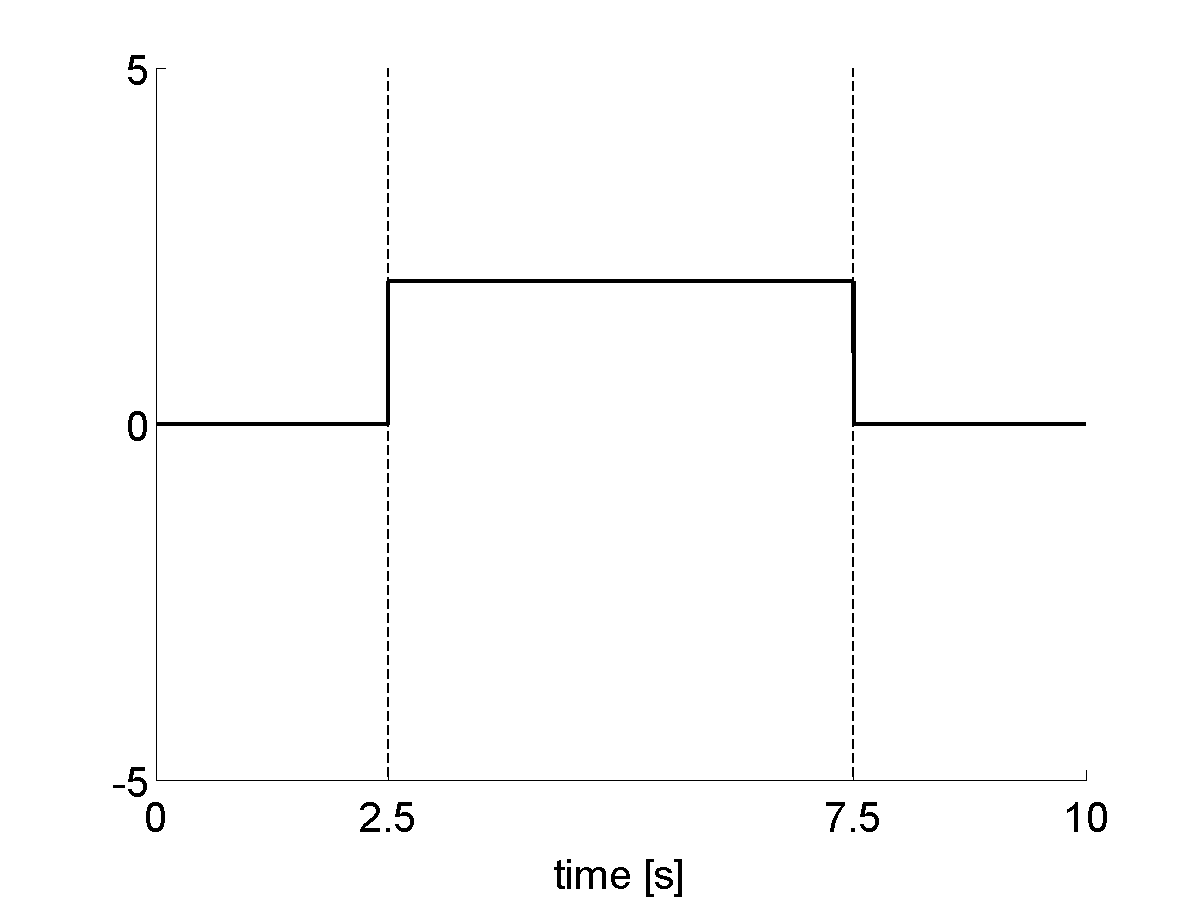
\includegraphics[width=0.5\textwidth]{stimgen/Documentation2009-img001.png}
\end{center}
\caption{DC elementary waveform}
\end{example}

\begin{example}
\begin{center}
\footnotesize\ttfamily
\begin{tabular}{rrrrrrrrrrrr}
2.5 & 1 & 0.0 & 0 & 0 & 0 & 0 & 0 & 0 & 0 & 0 & 1 \\
5.0 & 1 & -2.0 & 0 & 0 & 0 & 0 & 0 &0 & 0 & 0 & 1 \\
2.5 & 1 & 1.0 & 0 & 0 & 0 & 0 & 0 & 0 & 0 & 0 & 1 \\
\end{tabular}
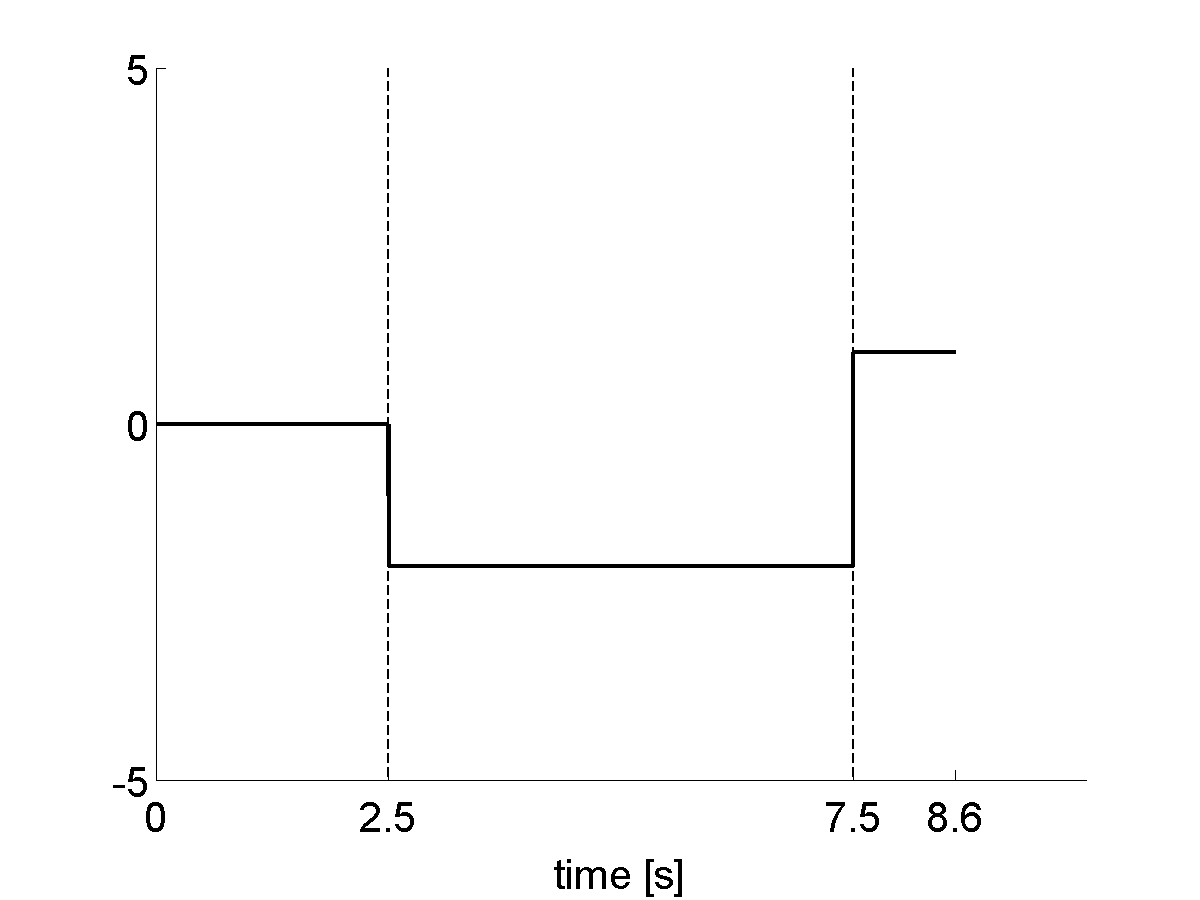
\includegraphics[width=0.5\textwidth]{stimgen/Documentation2009-img002.png}
\end{center}
\caption{DC elementary waveform}
\end{example}

\subsection{Ornstein-Uhlenbeck elementary waveforms}

\paragraph{}
The next elementary subwaveform is a (realization of a) stochastic process. The understanding of the underlying
mathematical details that accompany its definition needs some mathematical background that is not covered here (but see
the books by Cox \& Miller, or by Papoulis, on random variables and stochastic processes). The specific process we
consider here is the \textbf{Ornstein-Uhlenbeck process}, sometimes referred to as \textbf{colored noise}, or as
``exponentially-filtered'' white gaussian noise. A family of noisy subwaveforms (realizations) of this process can be
iteratively synthesized considering the following stochastic differential equation:

\begin{center}
$ df(t) = -f(t).dt/P_3 + dt P_1/P_3 + \xi_{t}.P_{2}(2\times dt/P_3)^{\frac{1}{2}}$ for all times $t \in [t_0:t_0 + T]$
\end{center}

\paragraph{}
We have indicated by $dt$ the sampling period (in \textit{ms)} and by $\xi_{t} $ the value returned
at each call by a routine for the computer-generation of a Gauss-distributed pseudo-random numbers, with zero-mean and
unitary variance. Internally, the library does not implement this specific iterative equation but another one that
allows an improved numerical precision. From mathematical considerations, it follows that for a certain (discrete)
sequence of $\xi_{t}$, $f(t)$ is a realisation of a stochastic process whose amplitude is gauss-distributed
with \textbf{mean} and \textbf{standard deviation} becoming time-invariant after a transient and equal to
\textbf{$P_1$} and \textbf{$P_2$}, at the steady-state respectively. In other words, the
distribution of the amplitudes of f(t) is non-stationary but after a (exponential) relaxation time (i.e. of the order
of \textbf{$P_3$}) it becomes stationary. The spectral properties of this
stochastic process are entirely specified by \textbf{$P_3$}, which is the
time-constant of the exponential function that represents the autocorrelation function of f(t). This parameter is
sometimes called \textbf{correlation length} of the process and it is always specified here in \textbf{ms}. 

\paragraph{}
As for the DC subwaveform, from the point of view of the user, only
\textbf{$P_1$}, \textbf{$P_2$}, and \textbf{$P_3$} need to be specified. As for the DC subwaveform, the
Orstein-Uhlenbeck process can be identified by the following string:

\begin{center}
\footnotesize\ttfamily
\begin{tabular}{rrrrrrrrrrrr}
[T & 2 & P1 & P2 & P3 & - & - & FIXSEED & MYSEED & - & - & EXPON]
\end{tabular}
\end{center}

\paragraph{}
For this particular subwaveform, given the internal use of a random number generator, there are other two additional
parameters under the user control: \textbf{FIXSEED }and \textbf{MYSEED}. When \textbf{FIXSEED} is set to 1 (i.e. its
accepted values are ``1'' or ``0'', as a logical variable), the seed of the internal random number generation algorithm
will be temporarily initialized to the integer specified by \textbf{MYSEED}. In order to confine the effect of
\textbf{FIXSEED }only to the current subwaveforms and not the subsequents, upon completion of the subwaveform
synthesis, the original seed at that point is restored. The consequences of several parameters choices are reported in
the examples.

\begin{example}
\begin{center}
\footnotesize\ttfamily
\begin{tabular}{rrrrrrrrrrrr}
0.1 & 1 & 0.0 & 0 & 0 & 0 & 0 & 0 & 0 & 0 & 0 & 1 \\
0.2 & 2 & -2.0 & 0.5 & 1 & 0 & 0 & 1 & 21 & 0 & 0 & 1 \\
0.05 & 1 & 0.0 & 0 & 0 & 0 & 0 & 0 & 0 & 0 & 0 & 1 \\
0.2 & 2 & 2.0 & 0.5 & 1 & 0 & 0 & 1 & 21 & 0 & 0 & 1 \\
0.1 & 1 & 0.0 & 0 & 0 & 0 & 0 & 0 & 0 & 0 & 0 & 1 \\
\end{tabular}
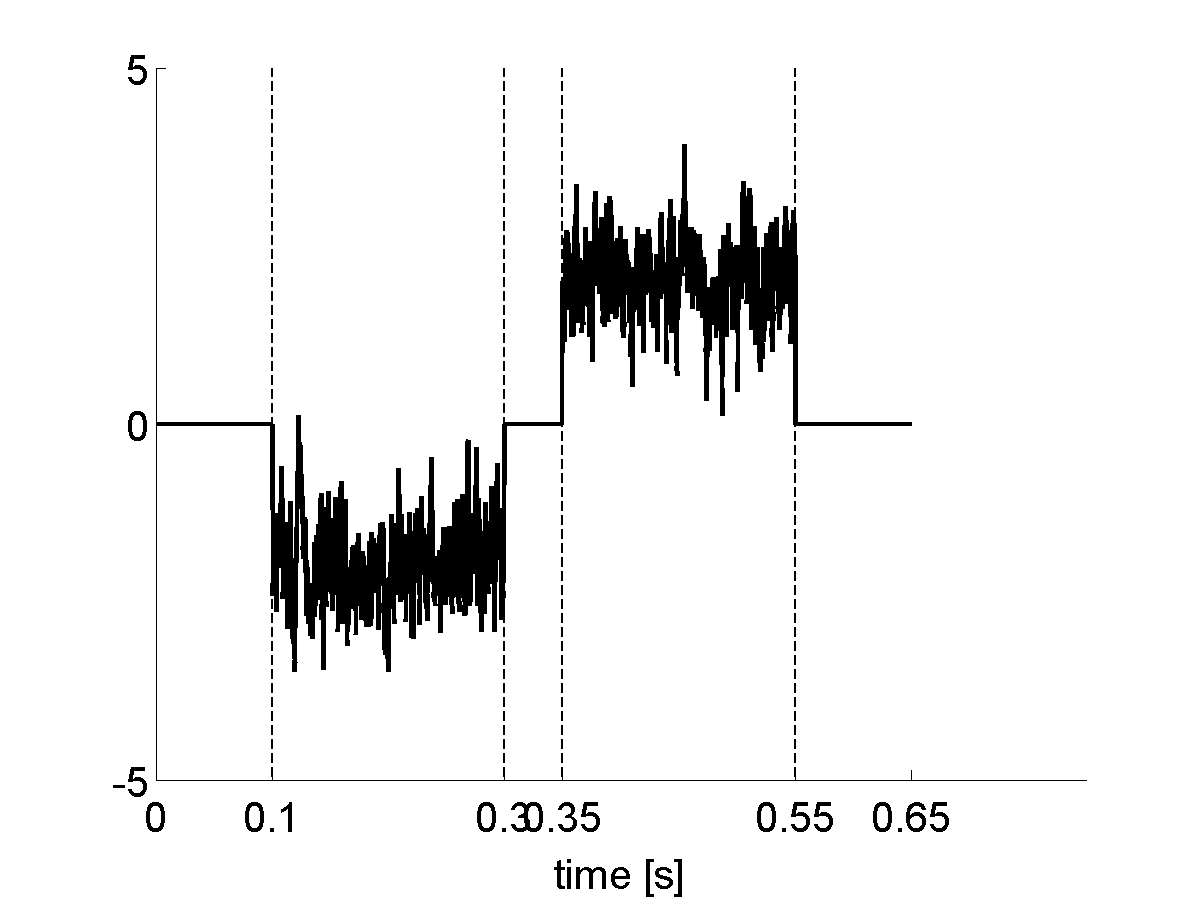
\includegraphics[width=0.5\textwidth]{stimgen/Documentation2009-img003.png}
\end{center}
\caption{Ornstein-Uhlenbeck elementary waveform}
\end{example}

\begin{example}
\begin{center}
\footnotesize\ttfamily
\begin{tabular}{rrrrrrrrrrrr}

0.1 & 1 & 0.0 & 0 & 0 & 0 & 0 & 0 & 0 & 0 & 0 & 1 \\
0.2 & 2 & 2.0 & 0.5 & 1 & 0 & 0 & 1 & 21 & 0 & 0 & 1 \\
0.05 & 1 & 0.0 & 0 & 0 & 0 & 0 & 0 & 0 & 0 & 0 & 1 \\
0.2 & 2 & 2.0 & 0.5 & 10 & 0 & 0 & 1 & 21 & 0 & 0 & 1 \\
0.1 & 1 & 0.0 & 0 & 0 & 0 & 0 & 0 & 0 & 0 & 0 & 1 \\
\end{tabular}
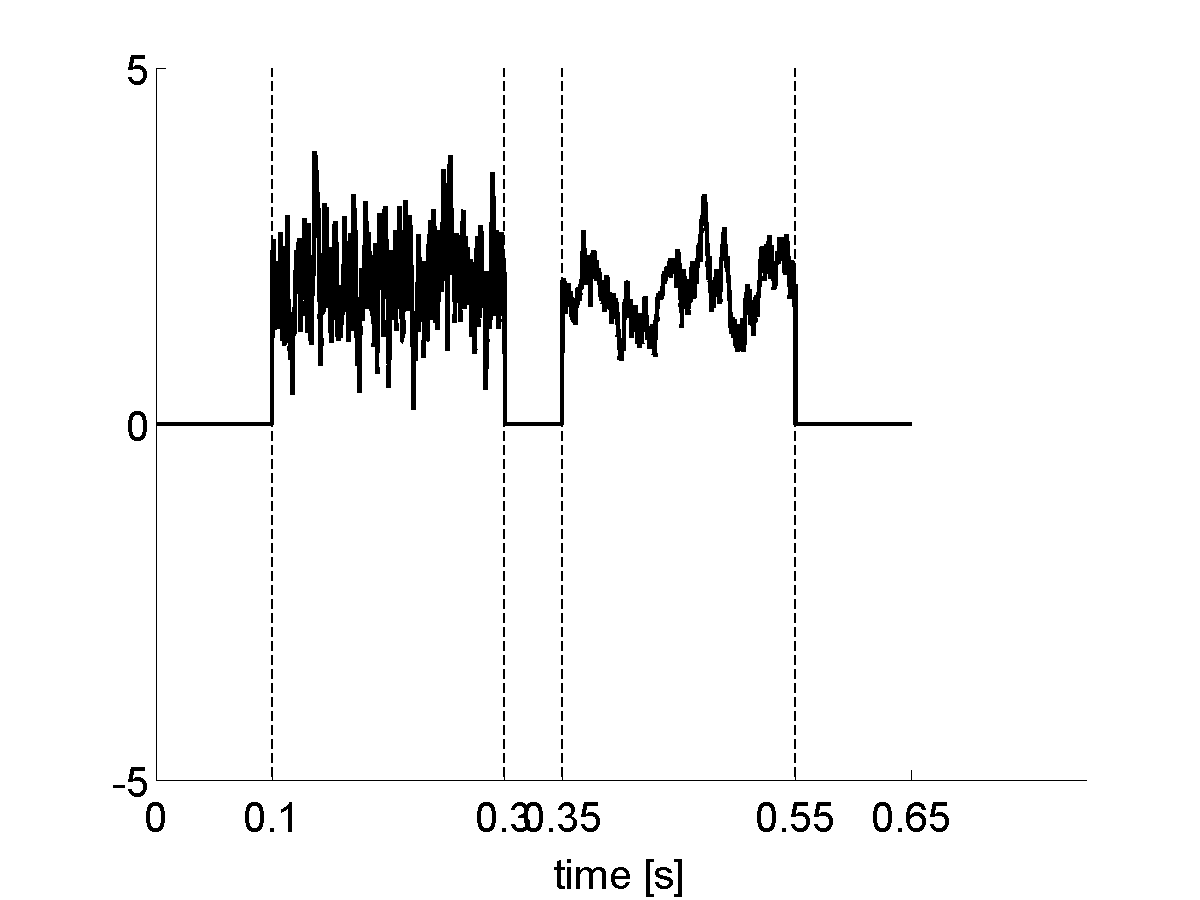
\includegraphics[width=0.5\textwidth]{stimgen/Documentation2009-img004.png}
\end{center}
\caption{Ornstein-Uhlenbeck elementary waveform}
\end{example}

\begin{example}
\begin{center}
\footnotesize\ttfamily
\begin{tabular}{rrrrrrrrrrrr}
0.1 & 1 & 0.0 & 0 & 0 & 0 & 0 & 0 & 0 & 0 & 0 & 1 \\
0.2 & 2 & 2.0 & 0.5 & 100 & 0 & 0 & 1 & 21 & 0 & 0 & 1 \\
0.05 & 1 & 0.0 & 0 & 0 & 0 & 0 & 0 & 0 & 0 & 0 & 1 \\
0.2 & 2 & 2.0 & 0.5 & 100 & 0 & 0 & 1 & 21 & 0 & 0 & 1 \\
0.05 & 1 & 0.0 & 0 & 0 & 0 & 0 & 0 & 0 & 0 & 0 & 1 \\
0.2 & 2 & 2.0 & 0.5 & 100 & 0 & 0 & 0 & 0 & 0 & 0 & 1 \\
0.1 & 1 & 0.0 & 0 & 0 & 0& 0 & 0 & 0 & 0 & 0 & 1 \\
\end{tabular}
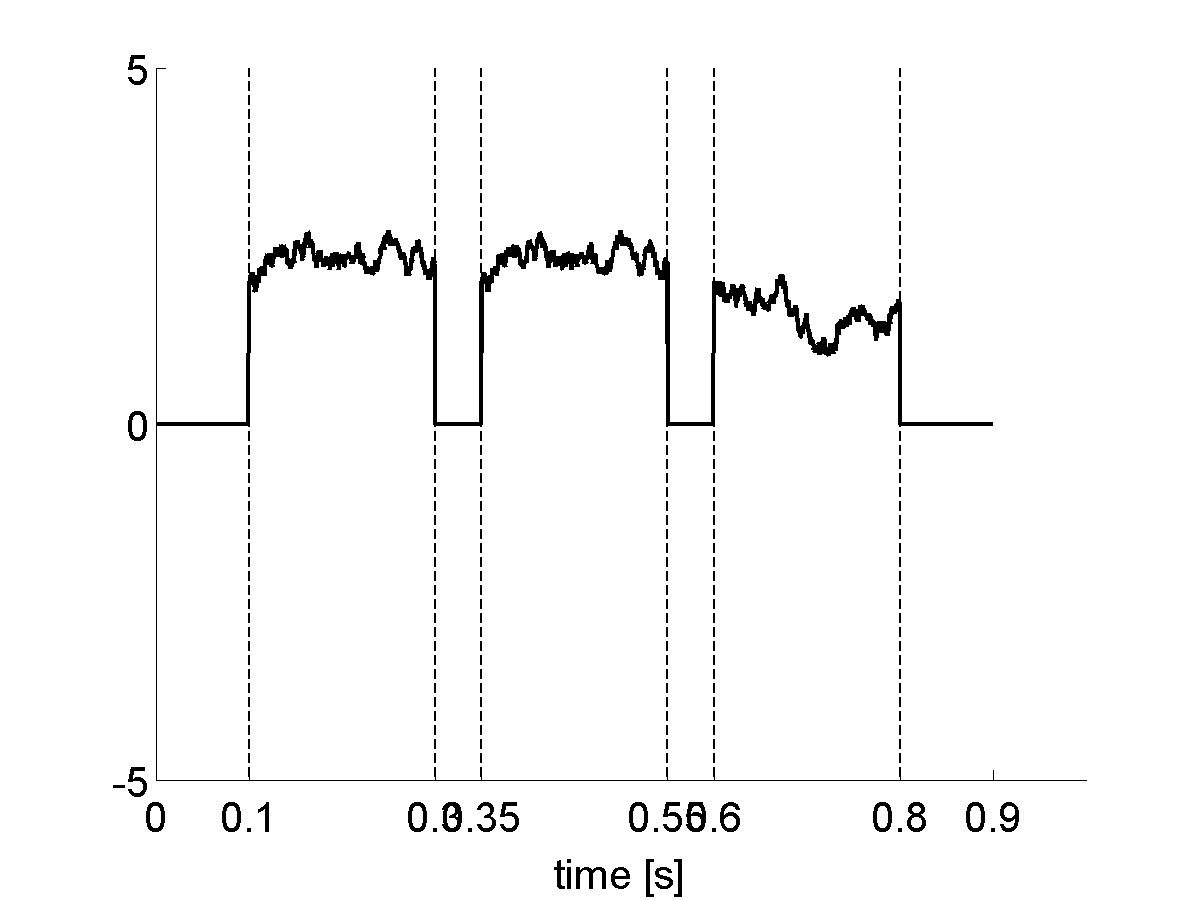
\includegraphics[width=0.5\textwidth]{stimgen/Documentation2009-img005.png}
\end{center}
\caption{Ornstein-Uhlenbeck elementary waveform}
\end{example}

